
\sektion{Lessons Learned}


%%%%%%%%%%%%%%%%%%%%%%%%%%%%%%%%%%%%%%%%%%%%%%%%
\begin{frame}
\frametitle{Kotlin is a great language}
\begin{itemize}
	\item Null handling is a MUST!
	\item Extension methods for better auto completion
	\item Named and default arguments, data classes
	\item Requires developers to be more disciplined
	\begin{itemize}
		\item Several classes in one (big) file gets common
		\item Overuse of single-expression functions
		\item Overuse of \texttt{apply\{\}}
		\item Explicit type declaration for documentation
	\end{itemize}
\end{itemize}
\end{frame}


%%%%%%%%%%%%%%%%%%%%%%%%%%%%%%%%%%%%%%%%%%%%%%%%
\begin{frame}
\frametitle{Tooling infrastructure grows}
\begin{itemize}
	\item Mostly same as for Java
	\item Build system support (gradle with kotlin coming!)
	\item Static code analysis tools missing
	\item Syntax highlighting mostly missing
\end{itemize}
\end{frame}

%%%%%%%%%%%%%%%%%%%%%%%%%%%%%%%%%%%%%%%%%%%%%%%%
\begin{frame}
\frametitle{IntelliJ support is quite good}
\begin{itemize}
	\item Auto convert from Java to Kotlin
	\item TODO2
	\item TODO3
	\item Automatic replace
\end{itemize}
\begin{figure}[h]
\centering
  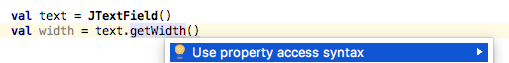
\includegraphics[width=10cm]{intellij_properties}
\end{figure}

\end{frame}

%* the "1-liner challenge": no references, just a = method
%* overdoing it with apply (who is this?)
%* data classes are restricted in usage => kotlin 1.1

